\section{Anwendung von Temporal-Difference Learning auf \ttt}
\label{sec:TDL_TTT}
Die folgenden Abschnitte behandeln die Umsetzung des Temporal-Difference Update und einer möglichen Rewardfunktion. 
Anschließend wird der Aufbau der Q-Tabelle erklärt und das Konzept der Afterstates eingeführt.

\subsection{Temporal-Difference Update und Rewardfunktion}

Zur Anwendung von \acl{RL} muss definiert werden, was die Bestandteile des \ac{MDP} sind. 
In \acl{TTT} entspricht das Spielfeld der Umgebung und ein Zustand $s$ ist eine Konstellation des Spielfeldes. 
Der Agent ist ein Spieler, der als Aktion einen freien Slot wählt, in dem das zugewiesene Symbol platziert wird. 
Die Menge der legalen Aktionen in einem Zustand $A(s)$ entspricht den unbelegten Slots auf dem Spielfeld. 
Ein Spiel kann aus maximal neun Zeitschritten bestehen und endet immer mit einem Ergebnis. 
\acs{TTT} gehört daher zu den episodischen \ac{RL} Problemen.

Die Abweichung von klassischen \ac{RL} Problemen ist, dass zwei Agenten abwechselnd Symbole platzieren. Da das klassische \ac{TDL} nicht für Multi-Agenten Probleme definiert ist, kann es nicht direkt angewendet werden \cite[S. 2f. ]{vanderreeReinforcementLearningGame2013}. 
Eine mögliche Lösung bietet die Agenten-Umgebung-Schnittstelle. 
Demnach kann der Gegner und dessen gewählte Aktionen als Teil der Umgebung betrachtet werden, da der Agent diesen nicht kontrolliert. 
Somit erhält der Agent von der Umgebung nur die Zustände, in denen er eine Aktion wählen kann.
Aus Sicht des Agenten ist \acs{TTT} eine stochastische Umgebung, da der Zug des Gegners und somit der nächste Zustand, den ein Agent erhält nicht deterministisch sind. \cite[S. 2f]{vanderreeReinforcementLearningGame2013}, \cite{soemersd.GameAiHow} 
Unter der Voraussetzung, dass X beginnt, können alle Zustände gerader Zeitschritte \bzw Symbolanzahl dem Agenten X und ungerade dem Agent O zugeordnet werden, wie in Abbildung \cref{fig:ttt_state_to_agent} dargestellt.
Die zugehörigen \ac{MDP} beziehen sich nun auf einen Agenten, sodass die vorgestellten Algorithmen angewendet werden können.

\begin{figure}
    \centering
    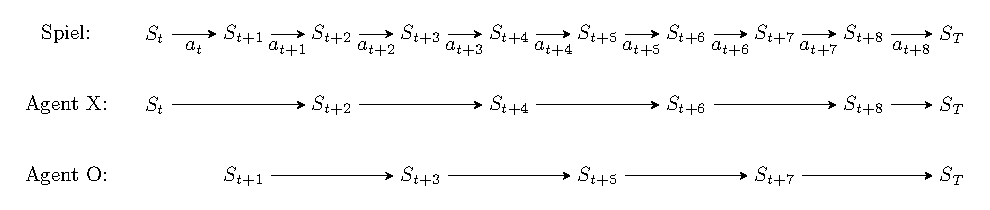
\includegraphics[width=\linewidth]{04_Artefakte/01_Abbildungen/ttt_state_to_agent.pdf}
    \caption{Zuordnung der \acs{TTT} Zustände und Zeitschritte zu den Agenten }
    \label{fig:ttt_state_to_agent}
\end{figure}

Für das \ac{TD} Update ist neben dem jetzigen Zustand $S_t$und der gewählten Aktion $a_t$ der nächste Zustand $S_{t+2}$, den der Agent erhält, notwendig. 
Da der nächste Zustand des Agenten abhängig von der Aktion des Gegners ist, erfolgt ein Update für einen Zustand erst, wenn der Gegner eine Aktion durchgeführt hat. 
Eine Besonderheit sind Terminalzustände, da diese das Spiel beenden und somit keine Aktion durch den Gegner möglich ist. 
Ein Terminalzustand $S_T$ wird erreicht, wenn ein Spieler eine Aktion wählt, durch die er das Spiel gewinnt oder in einem Unentschieden beendet. 
Wechselt ein Agent durch eine Aktion in einen Terminalzustand, wird dieser für das Update beider Agenten verwendet. \cite[S. 2f]{vanderreeReinforcementLearningGame2013}, \cite{soemersd.GameAiHow}
Dies ist möglich, da der \qValue jedes Terminalzustands per Definition 0 ist \cite[S. 74]{suttonReinforcementLearningIntroduction2018}. 
Die Unterscheidung, ob ein Spielergebnis gut oder schlecht für den Agenten ist, erfolgt im Update durch den Reward.

Beim Minimax-Algorithmus erhalten beide Symbole die gleiche Utility, weshalb es einen minimierenden und maximierenden Spieler gibt.
Die \ac{TD} Agenten hingegen versuchen ihren Return zu maximieren, sodass Reward positiv oder negativ, entsprechend des Spielergebnisses aus Agenten-Sicht sein muss.
\acs{TTT} ist ein Nullsummenspiel mit drei möglichen Spielergebnissen: Gewinn, Niederlage und Unentschieden.
Wie in \cref{sec:minimax} beschrieben, ist eine gängige Zuordnung $+1$, $-1$ und $0$.
Das Spielverhalten kann jedoch weiter differenziert werden durch Betrachtung der Spiellänge, gemessen in durchgeführten Aktionen. 
Ein optimaler Agent sollte versuchen, in möglichst wenigen Zügen zu gewinnen und eine Niederlage möglichst lange hinauszögern \cite[S. 533]{crowleyFlexibleStrategyUse1993}. 
Eine mögliche Umsetzung ist, den Reward je Spielzug in der Episode um $0.1$ gegen $0$ zu korrigieren.
Als Korrektur wird $0.1$ verwendet, da neun Spielzüge möglich sind und selbst bei Gewinn im letzten Zug ein positiver Reward zugewiesen wird.
Diese Korrektur wird im Folgenden als \gqq{Depth Penalty} bezeichnet, da eine Korrektur entsprechend der Tiefe (\engl depth) im Spielbaum erfolgt.
Dieser Reward bewertet, ob der Agent das Ziel, \acs{TTT} zu Gewinnen, erreicht hat und wird daher als letzter Reward einer Episode ausgeteilt.
Die Rewards aller anderen Aktionen sind 0, da deren Bedeutung für das Spielergebnis nicht bekannt ist. 
Der Reward kann somit mittels \cref{eq:depth_penalty} berechnet werden und  liefert die in \cref{tab:reward_depth_penalty} gelisteten Rewards.
Da der unkorrigierte Reward für Sieg und Niederlage $1$ und $-1$ ist, kann er genutzt werden, um das Vorzeichen der Korrektur anzupassen.
Andere Definitionen eines Rewards sind möglich, werden in dieser Arbeit jedoch nicht betrachtet \cite{mirnovi.QLearningTicTacToe2020}.

\begin{equation}\label{eq:depth_penalty}\equationentry{Formel für korrigierten Reward mit Depth Penalty}
   \text{reward}_{\text{angepasst}}= \text{reward}- (\text{reward}\cdot \text{depth} \cdot 0,1)
\end{equation}

\begin{table}
\centering
\caption{Mögliche Rewards pro Spielzug bei Korrektur des Rewards mittels Depth Penalty}
\label{tab:reward_depth_penalty}
\begin{tabular}{lrr}
\toprule
 Zug   & Reward Agent  & Reward Gegner \\ \midrule
1      & /              & / \\
2      & /              & / \\
3      & /              & / \\
4      & /              & / \\
5      & 0,5            & -0,5\\
6      & -0,4           & 0,4 \\
7      & 0,3            & -0,3\\
8      & -0,2           & 0,2 \\
9      & 0,1            & -0,1 \\ \bottomrule
\end{tabular}
\end{table}


\subsection{\qtable und Kompression durch Afterstates}
\label{sec:afterstates}

Die \qtable enthält die Abbildung der \ac{SA Tupel} auf einen \qValue. 
Da jeder Zustand und somit jedes \ac{SA Tupel} eindeutig einem Symbol zugeordnet werden kann, können die \qValues für beide Symbole in einer gemeinsamen \qtable gespeichert werden. 
Wird die \qtable als eine Lookup-Tabelle visualisiert, wie in \cref{tab:qtable_example}, enthält diese für jeden der 5478 Zustände eine Zeile. 
Die Aktionen sind die Spalten, wobei die Aktionen nicht für jeden Zustand gleich sind, sondern den freien Slots auf dem Spielfeld entsprechen.

\begin{table}
\centering
\caption[Q-Tabelle für \acs{TTT}]{\qtable für \acs{TTT}. $S_{5477}$ ist ein Beispiel für einen Terminalzustand, in dem keine Aktionen möglich sind, dargestellt durch \gqq{/}}
\label{tab:qtable_example}
\begin{tabular}{lllll}
\toprule
State       &   $a_0$           &   $a_1$       & $\dots$   & $a_8$         \\ \midrule
$S_0$       &   $Q(S_0,a_0)$    &  $Q(S_0,a_1)$ & $\dots$   & $Q(S_0,a_8)$  \\
$S_1$       &   $Q(S_1,a_0)$    &  $Q(S_1,a_1)$ & $\dots$   & $Q(S_1,a_8)$  \\
$\vdots$    & $\vdots$          & $\vdots$      & $\ddots$  & $\vdots$      \\
$S_ {5477}$    &  /                 &  /           & $\dots$   & /  \\ \bottomrule
\end{tabular}
\end{table}


Wie im vorigen Abschnitt  beschrieben, besteht eine Runde aus einem deterministischen Zustandswechsel durch den Agenten und einem stochastischen Zustandswechsel durch die Umgebung.
In \acs{TTT} können unterschiedliche \ac{SA Tupel} dieselbe Spielfeldkonstellation erzeugen, bevor der Gegner zum Zug kommt, wie in \cref{fig:ttt_afterstate} dargestellt. 
Die Zustände nach dem deterministischen Zustandswechsel durch den Agenten werden als Afterstate (\dt Folgezustand) bezeichnet und können als surjektive Abbildung der \ac{SA Tupel} auf die Menge der Afterstates $Y$ beschrieben werden: $(S,A) \rightarrow Y$.  
\ac{SA Tupel}, die denselben Afterstate haben, sollten einen gemeinsamen \qValue besitzen. 
Dadurch wird Erfahrung, die durch ein \ac{SA Tupel} gesammelt wird, mit den anderen geteilt, sodass der Lernprozess beschleunigt wird. \cite[S. 136f.]{suttonReinforcementLearningIntroduction2018}

\begin{figure}
    \centering
    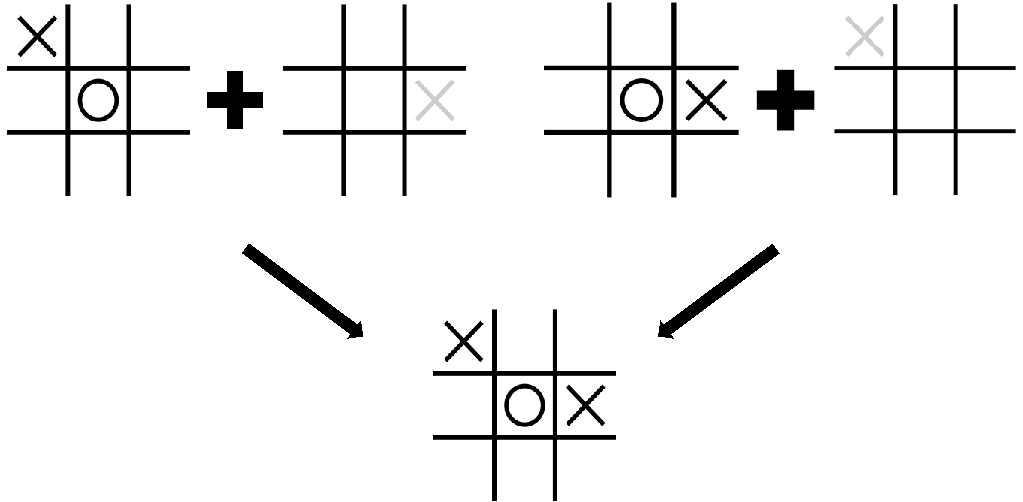
\includegraphics[scale=0.4]{04_Artefakte/01_Abbildungen/ttt_boards/ttt_afterstate.pdf}
    \caption[Beispiel für Afterstates in \acs{TTT}]{Beispiel für Afterstates in \acs{TTT}. Zwei \ac{SA Tupel} können im selben Afterstate resultieren \protect\footnotemark}
    \label{fig:ttt_afterstate}
\end{figure}

\footnotetext{Abbildung entnommen aus \cite[S. 137]{suttonReinforcementLearningIntroduction2018}}
Mit der vorgestellten \qtable ist dies jedoch nicht möglich, da die \qFunction jedem \ac{SA Tupel} einen individuellen \qValue zuweist und der resultierende Zustand dem anderen Symbol zugeordnet ist. 
Daher wird eine \afterStateVFunction genutzt, die statt einem \ac{SA Tupel} $(S,A)$ dem resultierenden Afterstate $y$ einen Wert zuweist. 
Der zugewiesene Wert kann, zur Unterscheidung vom \qValue, als \wValue $w$ bezeichnet werden.\cite{nbroReinforcementLearningHow}

Ein Agent wählt nun in einem Zustand, die Aktion, die im Afterstate mit dem höchsten \wValue resultiert. 
Die bisherige \qtable wird geteilt in zwei separate Tabellen, wie in  \cref{tab:afterstate} und \cref{tab:wtable} dargestellt. 
Einerseits die surjektive Abbildung $(S,A) \rightarrow Y$ sowie die Zuweisung des \wValue zu einem Afterstate: $y \rightarrow w$, die im Folgenden als \afterstateTable und \wtable bezeichnet werden. 
Im Gegensatz zur \qtable umfasst der \wtable nur 5477 Zeilen, da der Ausgangszustand kein Afterstate ist. 
Die Anzahl der \wValues ist im Vergleich zur Anzahl von \qValues deutlich komprimiert, da \ac{SA Tupel}, die denselben Afterstate $y$ haben einen \wValue teilen.
Streng genommen benötigt ein Agent mit \afterStateVFunction nur die Menge der erreichbaren Afterstates und nicht den Zustand oder die legalen Aktionen selbst, da diese durch die Abbildung $(S,A) \rightarrow Y$ implizit enthalten sind. \cite{nbroReinforcementLearningHow}

\begin{table}[!htb]
    \begin{minipage}{.5\textwidth}
        \centering
        \caption{\afterstateTable für \acs{TTT}}
        \label{tab:afterstate}
        \begin{tabular}{lllll}
        \toprule
        State       & $a_0$     & $a_1$     & $\dots$     & $a_8$   \\ \midrule
        $S_0$       & $y_0$     & $y_1$     & $\dots$     & $y_8$   \\
        $S_1$       & $y_1$     & $y_0$     & $\dots$     & $\dots$ \\
        $\vdots$    & $\vdots$  & $\vdots$  & $\ddots$    & $\vdots$ \\
        $S_{5477}$  & $\dots$   & $\dots$   & $\dots$    &  $\dots$\\ \bottomrule
        \end{tabular}
    \end{minipage}%
    \begin{minipage}{.5\textwidth}
        \centering
        \caption{\wtable für \acs{TTT}}
        \label{tab:wtable}
        \begin{tabular}{ll}
        \toprule
        Afterstate  & \wValue       \\ \midrule
        $y_0$       & $w(y_o)$      \\
        $y_1$       & $w(y_1)$      \\
        $\vdots$    & $\vdots$      \\
        $y_{5476}$  & $w(y_{5476})$ \\ \bottomrule
        \end{tabular}
    \end{minipage}
\end{table}

